\chapter{Benchmark}
This section does concerned with a benchmark between the two databases PostgreSQL 9.6, PostgreSQL 10.0 and MapD CE 3.0.
The dataset is based on a part of the New York City Taxi and Limousine Commission (TLC) Trip Record Data \cite{nyc}.
All queries were executed on the same server.

\section{Dataset}
\label{sec:dataset}
\begin{figure}[H]
\centering
\captionsetup{justification=centering}
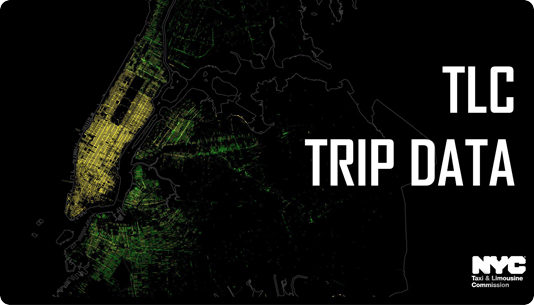
\includegraphics[width=0.9\textwidth]{images/nyc_taxi.png}
\caption[Taxi Dropoffs]{TLC Trip Record Data}
\end{figure}

The New York City Taxi and Limousine Commission (TLC) Trip Record Data \cite{nyc} consists of trip records from the yellow and green taxis.
Furthermore there are data from the For-Hire Vehicle (FHV).
The data includes information about capturing pick-up and drop-off locations, times, trip distances, fares, rate types, and driver-reported passenger counts.

To simplify the handling with the huge amount of data we used the scripts from the Github repository \cite{nyctaxigithub}, that is able to download all the data,
provides the schema for PostgreSQL with the PostGIS \cite{postgis} extension and consists of scripts to import the data.

\subsection{Specification}
To get a brief overview of the specification have a look at the following list.
\begin{itemize}[noitemsep, topsep=0pt]
\itemsep-0.5em
 \item[Format:]  CSV
 \item[Yellow:]  January 2009 - June 2017
 \item[Green:]  August 2013 - June 2017
 \item[FHV:]  January 2015 - June 2017
 \item[Taxi trips:] Over 1.1 billion \cite{billion}
 \item[Size:] 267 GB \cite{billion}
\end{itemize}

\subsection{Data subset}
Due to the fact that not all GPU databases are able to handle queries based on data larger than the GPU memory,
we had to shrink the dataset fitting into the available memory.

The GPU used on the server for the benchmark is a Nvidia Tesla K40m with 12 GB memory.
Hence we used the yellow and green taxi trip data of the year 2015, that has a size of 25 GB, too.
Consequently all queries fit into the GPU memory.


\newpage
\section{Queries}
\label{sec:queries}
The Queries were predefined by Prof. Stefan Keller and are inspired by the Google BigQuery examples \cite{bigquery}.
All the queries are listed below, the used syntax is able to run on MapD. \\


\begin{lstlisting}[language=sql, caption={Query 1, Counts all the yellow taxi trips},captionpos=b]
SELECT cab_type_id, Count(*)
FROM   trips
GROUP  BY 1;
\end{lstlisting}


\begin{lstlisting}[language=sql, caption={Query 2, Calculates the average passenger amount per trip},captionpos=b]
SELECT passenger_count, Avg(total_amount)
FROM   trips
GROUP  BY 1;
\end{lstlisting}

\begin{lstlisting}[language=sql, caption={Query 3, Sums the yearly amount of passengers},captionpos=b]
SELECT passenger_count, Extract(year FROM pickup_datetime), Count(*)
FROM   trips
GROUP  BY 1, 2;
\end{lstlisting}


\begin{lstlisting}[language=sql, caption={Query 4, Groups the amount of passenger by year regarding the trip distance},captionpos=b]
SELECT passenger_count, Extract(year FROM pickup_datetime), Cast(trip_distance AS INT), Count(*)
FROM   trips
GROUP  BY 1, 2, 3
ORDER  BY 2, 4 DESC;
\end{lstlisting}

\begin{lstlisting}[language=sql, caption={Query 5, Queries all trips in a certain bounding box},captionpos=b]
SELECT *
FROM   trips
WHERE  ( pickup_longitude BETWEEN -74.007511 AND -73.983479 )
       AND ( pickup_latitude BETWEEN 40.7105 AND 40.731071 ) LIMIT 10;
\end{lstlisting}


\begin{lstlisting}[language=sql, caption={Query 6, Determines the average speed of the yellow taxi trips by hour of the day in a bounding box},captionpos=b]
SELECT Extract(HOUR FROM pickup_datetime) AS h, AVG(trip_distance / NULLIF(TIMESTAMPDIFF(HOUR,pickup_datetime, dropoff_datetime),0)) AS speed
FROM   trips
WHERE  ( pickup_longitude BETWEEN -74.007511 AND -73.983479 )
       AND ( pickup_latitude BETWEEN 40.7105 AND 40.731071 )
       AND trip_distance > 0
       AND fare_amount / trip_distance BETWEEN 2 AND 10
       AND dropoff_datetime > pickup_datetime
       AND cab_type_id = 1
GROUP  BY h
ORDER  BY h;
\end{lstlisting}


\begin{lstlisting}[language=sql, caption={Query 7, Computes the average speed of the yellow taxi trips by hour of the day},captionpos=b]
SELECT Extract(HOUR FROM pickup_datetime) AS h, Avg(trip_distance / NULLIF(TIMESTAMPDIFF(HOUR, pickup_datetime, dropoff_datetime),0))AS speed
FROM   trips
WHERE  trip_distance > 0
       AND fare_amount / trip_distance BETWEEN 2 AND 10
       AND dropoff_datetime > pickup_datetime
       AND cab_type_id = 1
GROUP  BY h
ORDER  BY h;
\end{lstlisting}


\begin{lstlisting}[language=sql, caption={Query 8, Calculates the average speed of the yellow taxi trips by day of the week},captionpos=b]
SELECT Extract(DOW FROM pickup_datetime) AS dow, Avg(trip_distance / NULLIF(TIMESTAMPDIFF(HOUR,pickup_datetime,  dropoff_datetime), 0)) AS speed
FROM   trips
WHERE  trip_distance > 0
       AND fare_amount / trip_distance BETWEEN 2 AND 10
       AND dropoff_datetime > pickup_datetime
       AND cab_type_id = 1
GROUP  BY dow
ORDER  BY dow;
\end{lstlisting}


\begin{lstlisting}[language=sql, caption={Query 9, Determines the average speed of the yellow taxi trips by day of the week in a bounding box},captionpos=b]
SELECT Extract(DOW FROM pickup_datetime) AS dow, Avg(trip_distance / NULLIF(TIMESTAMPDIFF(HOUR,pickup_datetime,  dropoff_datetime), 0)) AS speed
FROM   trips
WHERE  ( pickup_longitude BETWEEN -74.007511 AND -73.983479 )
       AND ( pickup_latitude BETWEEN 40.7105 AND 40.731071 )
       AND trip_distance > 0
       AND fare_amount / trip_distance BETWEEN 2 AND 10
       AND dropoff_datetime > pickup_datetime
       AND cab_type_id = 1
GROUP  BY dow
ORDER  BY dow;
\end{lstlisting}

\newpage
\section{Results}
As already mentioned the queries of the benchmark were applied on a database without GPU acceleration,
in our case PostgreSQL 9.6 and PostgreSQL 10.0.
Furthermore on MapD CE 3.0 a GPU powered database.
The dataset was introduced in section~\ref{sec:dataset} and the queries are listed in the section~\ref{sec:queries}.
The benchmark has been executed on a server with the specifications as you can see in table \ref{tab:hardware}.


\begin{table}[H]
\centering
\begin{tabular}{|l|l|}
\hline
CPU & Intel XEON E5-2670 v2 @ 2.50GHz (40 cores)\\ \hline
GPU & Nvidia Tesla K40m (12 GB)\\ \hline
RAM & 512 GB\\
\hline
\end{tabular}
\caption{Hardware specification}
\label{tab:hardware}
\end{table}

\subsection{Charts}
The following bar charts show the results of the benchmark.
For each query there is chart and chart has six bars.
There are two bars for each database, one for the first time of execution (cold) and one for the mean of the next 5 executions (warm).
For PostgreSQL we used the pg\_prewarm extension to load the data into the memory for the warm execution.

\begin{figure}[H]
    \centering
    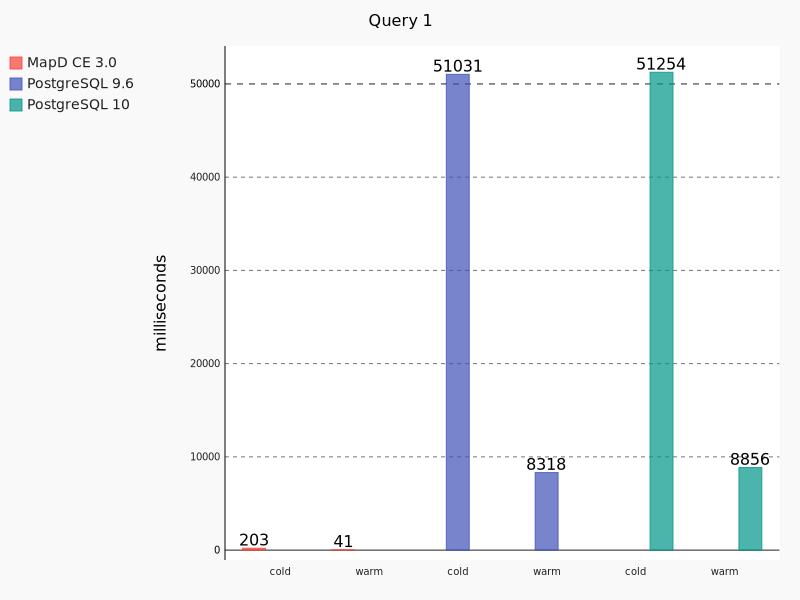
\includegraphics[width=0.9\textwidth,keepaspectratio]{charts/query_1.png}
    \caption{Query 1}
    \label{fig:query_1}
\end{figure}

\begin{figure}[H]
    \centering
    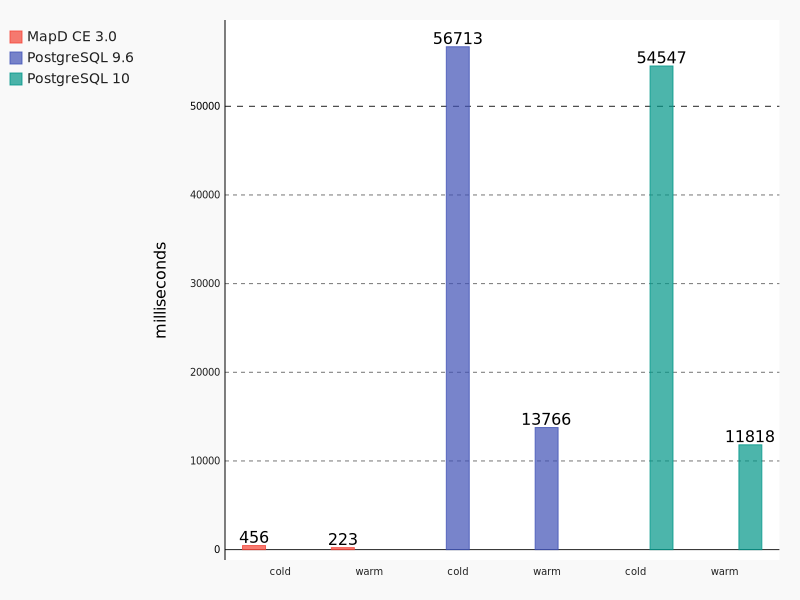
\includegraphics[width=0.9\textwidth,keepaspectratio]{charts/query_2.png}
    \caption{Query 2}
    \label{fig:query_2}
\end{figure}


\begin{figure}[H]
    \centering
    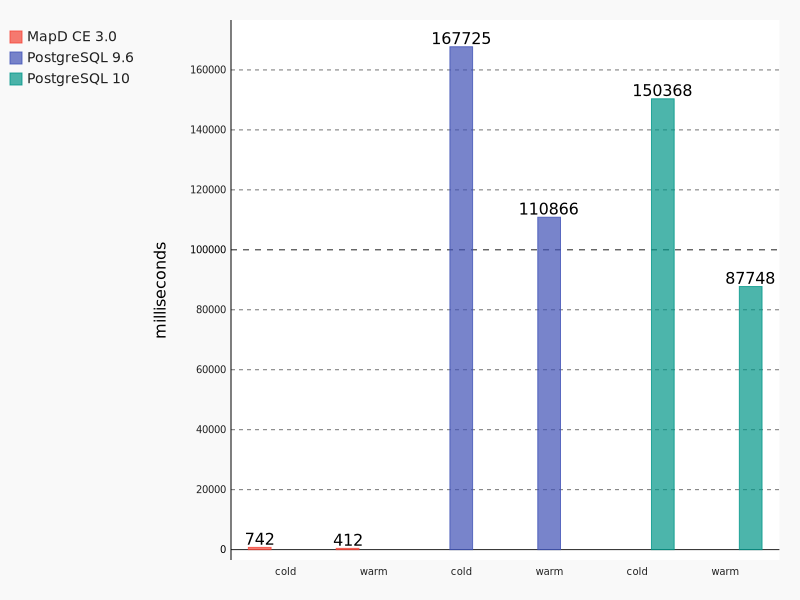
\includegraphics[width=0.9\textwidth,keepaspectratio]{charts/query_3.png}
    \caption{Query 3}
    \label{fig:query_3}
\end{figure}


\begin{figure}[H]
    \centering
    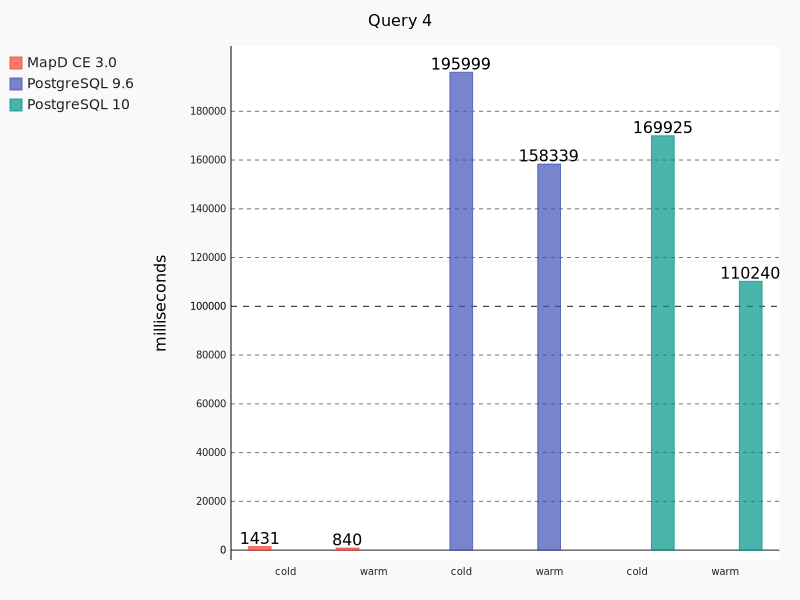
\includegraphics[width=0.9\textwidth,keepaspectratio]{charts/query_4.png}
    \caption{Query 4}
    \label{fig:query_4}
\end{figure}

\begin{figure}[H]
    \centering
    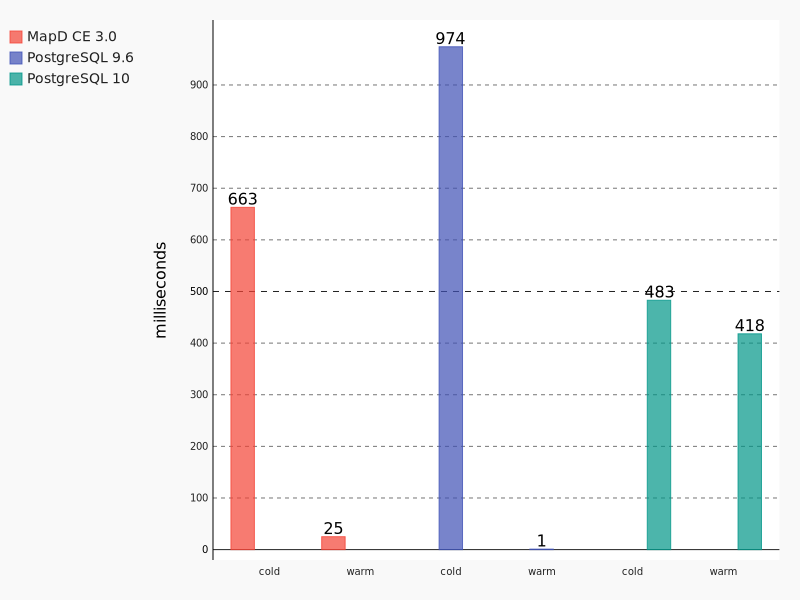
\includegraphics[width=0.9\textwidth,keepaspectratio]{charts/query_5.png}
    \caption{Query 5}
    \label{fig:query_5}
\end{figure}

\begin{figure}[H]
    \centering
    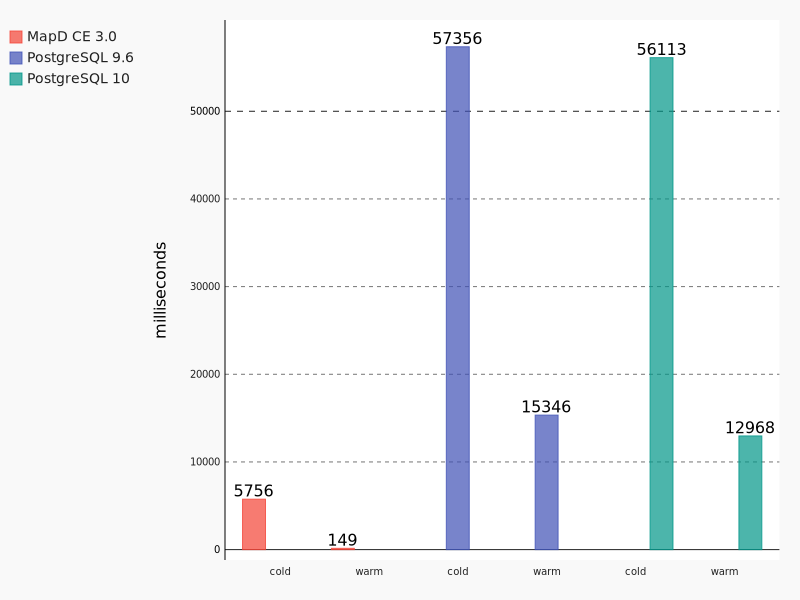
\includegraphics[width=0.9\textwidth,keepaspectratio]{charts/query_6.png}
    \caption{Query 6}
    \label{fig:query_6}
\end{figure}

\begin{figure}[H]
    \centering
    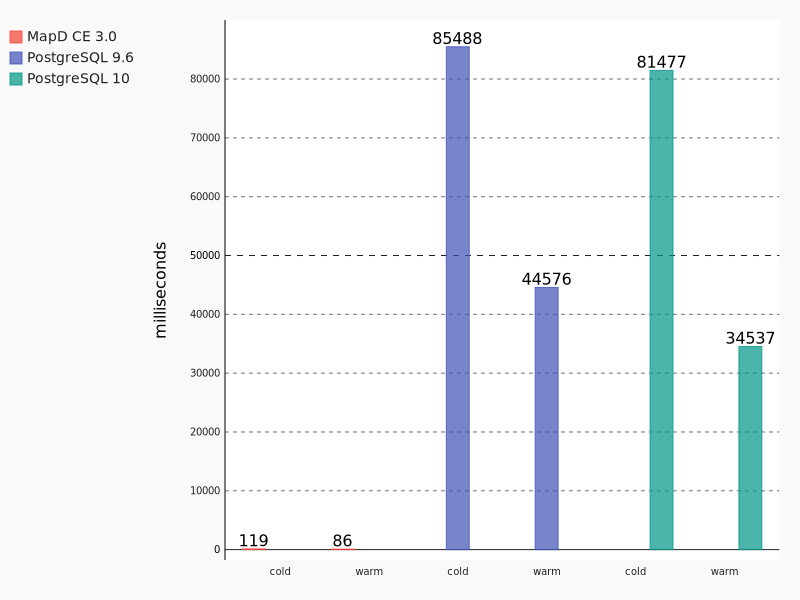
\includegraphics[width=0.9\textwidth,keepaspectratio]{charts/query_7.png}
    \caption{Query 7}
    \label{fig:query_7}
\end{figure}

\begin{figure}[H]
    \centering
    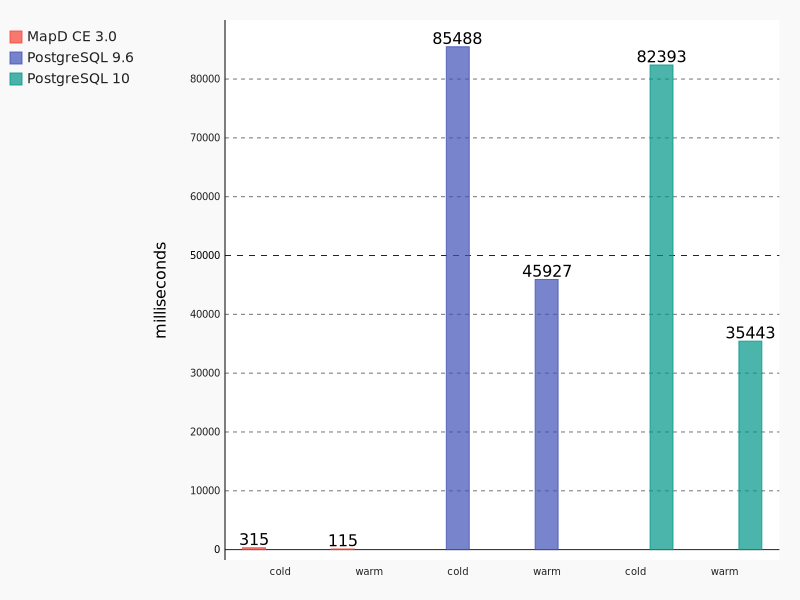
\includegraphics[width=0.9\textwidth,keepaspectratio]{charts/query_8.png}
    \caption{Query 8}
    \label{fig:query_8}
\end{figure}

\begin{figure}[H]
    \centering
    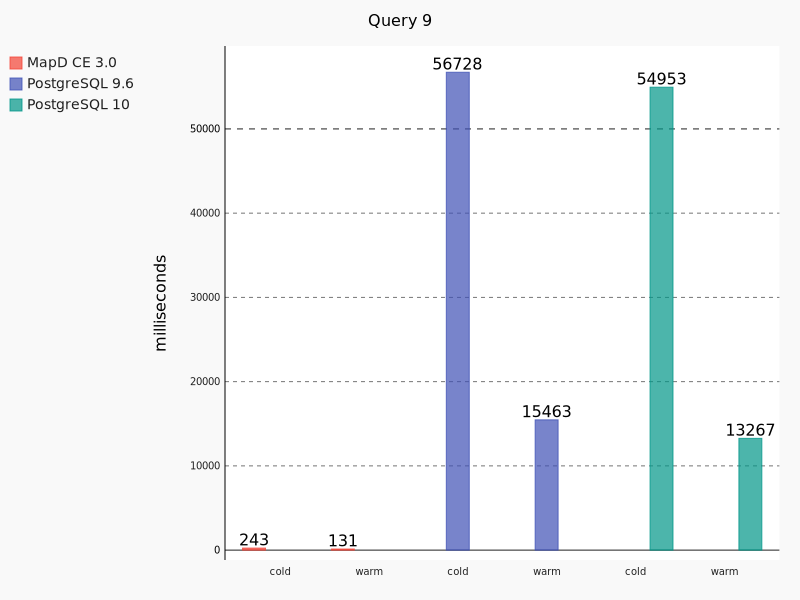
\includegraphics[width=0.9\textwidth,keepaspectratio]{charts/query_9.png}
    \caption{Query 9}
    \label{fig:query_9}
\end{figure}

\subsection{Data}
The table \ref{tab:data} show the results of the queries in tabular format. The unit of the numbers is milliseconds.
\begin{table}[H]
\centering
\begin{tabular}{|p{1.2cm}|p{2cm}|p{2cm}|p{2cm}|p{2cm}|p{2cm}|p{2cm}|}
\hline
Query & MapD cold & MapD warm & Postgres 9.6 cold & Postgres 9.6 warm & Postgres 10 cold & Postgres 10 warm \\
\hline
1 & 203 & 41 & 51031 & 8318 & 51254 & 8856 \\
2 & 456 & 223 & 56713 & 13766 & 54547 & 11818 \\
3 & 742 & 412 & 167725 & 110866 & 150368 & 87748 \\
4 & 1431 & 840 & 195999 & 158339 & 169925 & 110240 \\
5 & 663 & 25 & 974 & 1 & 483 & 418 \\
6 & 5756 & 149 & 57356 & 15346 & 56113 & 12968 \\
7 & 119 & 86 & 85488 & 44576 & 81477 & 34537 \\
8 & 315 & 115 & 88437 & 45927 & 82393 & 35443 \\
9 & 243 & 131 & 56728 & 15463 & 54953 & 13267 \\
\hline
\end{tabular}
\caption{Data}
\label{tab:data}
\end{table}

\subsection{Explain and analyse}
PostgreSQL provides the possibility to show the execution plan.
And an interesting fact is that no query used more than 8 workers.
An example is displayed at figure \ref{fig:explain}.

\begin{figure}[H]
    \centering
    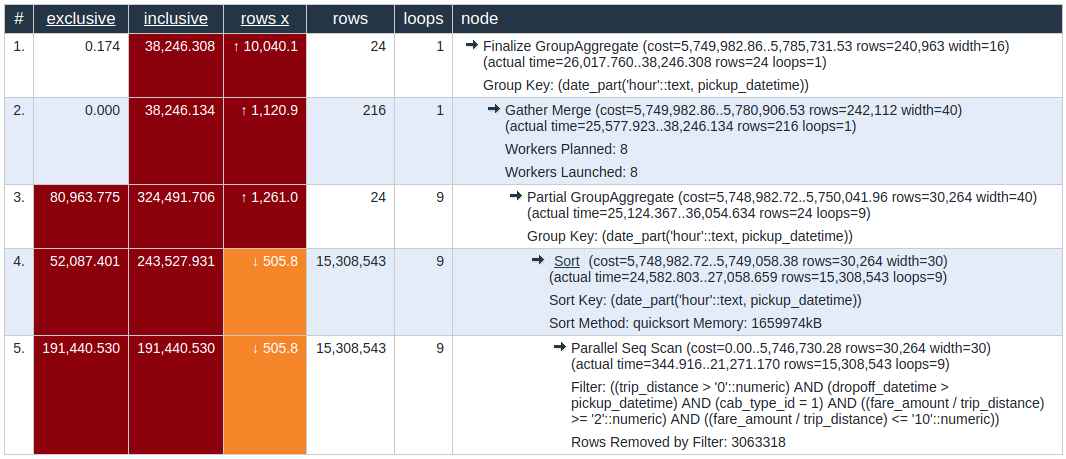
\includegraphics[width=1\textwidth,keepaspectratio]{images/explain_p10_q7.png}
    \caption{Explain and analysem, PostgresSQL 10}
    \label{fig:explain}
\end{figure}

Several attempts didn't lead to a higher degree of parallelism.
To reproduce the achieved results there are the configurations of the PostgreSQL database at section \ref{sec:config}.

\newpage
\subsection{Conclusion}
MapD is on nearly every query faster than PostgreSQL 9.6 and PostgreSQL 10.
Only on query 5 as you can see in figure \ref{fig:query_5} PostgreSQL is more performant the MapD.
Since there is a LIMIT statement in the query and PostgreSQL is able to stop after the limit is reached.
The performance of MapD is really astonishing.
The huge speedup compared to PostgreSQL might due to the fact that MapD is an in-memory database and the GPU acceleration is a big improvement as well.
Further, the MapD usage of a column store instead of a row-oriented storage like PostgreSQL does increase the performance, too.
And the fact that MapD is developed for an analytical purpose and doesn't support transaction in contrast to PostgreSQL must not be forgotten.
Another interesting insight can be observed at the comparison of the query execution at the first time (cold) or the following executions (warm).
The pg\_prewarm extension accelerate the PostgreSQL massively.
